\documentclass[]{article}

%opening
\title{4F13 Probabilistic Machine Learning - Latent Dirichlet Allocation}
\author{Candidate: 5562E}

%packages
\usepackage[margin=0.5in]{geometry}
\usepackage[export]{adjustbox}
\usepackage{mathtools}
\usepackage{graphicx}
\usepackage{amsmath}
\usepackage{amssymb}
\usepackage{hyperref}
\usepackage{caption}
\usepackage{subcaption}
\usepackage{parskip}
\usepackage{listings}
\usepackage{pdfpages}
\usepackage{bbm}

%package setup
\graphicspath{{./img/}}
\DeclareMathOperator*{\argmax}{arg\,max}
\DeclareMathOperator*{\argmin}{arg\,min}

%custom commands
\newcommand{\Fcal}{\mathcal{F}}
\newcommand{\idft}{\mathcal{F}^{-1}}
\newcommand{\Xcal}{\mathcal{X}}
\newcommand{\Ncal}{\mathcal{N}}
\newcommand{\Acal}{\mathcal{A}}
\newcommand{\Bcal}{\mathcal{B}}
\newcommand{\cmplx}{\mathbb{C}}
\newcommand{\Lcal}{\mathcal{L}}
\newcommand{\Mcal}{\mathcal{M}}
\newcommand{\indep}{\perp \!\!\! \perp}
\newcommand{\iid}{\stackrel{iid}{\sim}}
\newcommand{\figwidth}{0.6\linewidth}
\newcommand{\betaml}{\hat{\beta}^{ML}}
\newcommand{\Expect}{\mathbb{E}}


%section numbering
\renewcommand{\thesubsection}{\alph{subsection}}

\begin{document}

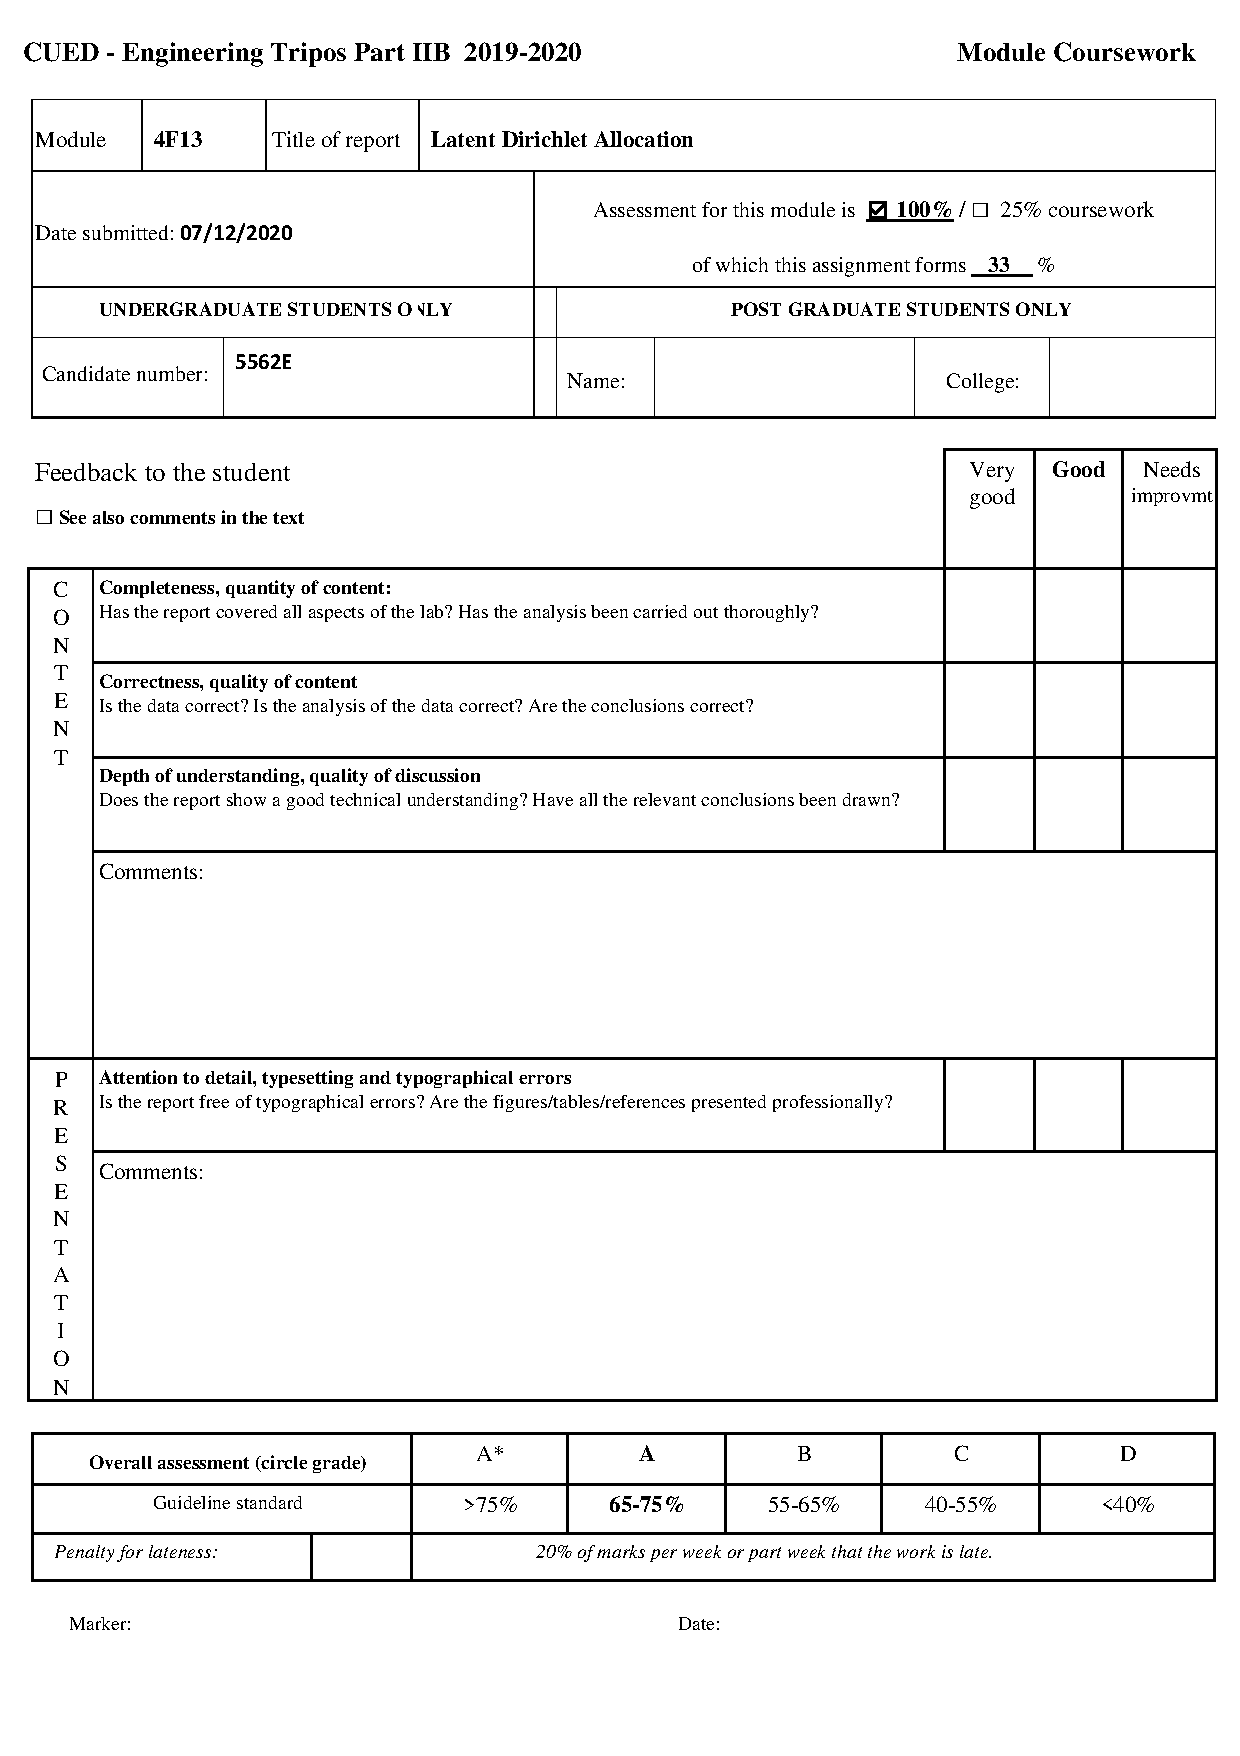
\includepdf[pages={1}]{coversheet-CW3.pdf}

\setcounter{page}{1}
\maketitle

\tableofcontents

\section{Introduction}

We have a document test set $\Acal$, which consists of $D$ documents indexed by $d \in \{1 \dots D\}$. A document is an ordered list of words. The vocabulary $\Mcal$ has $M=|\Mcal|$ unique words. We denote the $n$'th word in the $d$'th document by $w_{nd} \in \{1 \dots N_d\}$. Where $N_d$ is the length of document $d$. For simplicity we denote the count of occurrences of word $m$ in the training set by $c_m$.

We hold back a test set $\Bcal$ to calculate the performance of our approaches.

\section{Questions}
\subsection{Maximum Likelihood}

We begin by assuming that each word is drawn independently from a categorical distribution with parameter $\beta$: $w_{nd} \iid Cat(\beta)$. In this case $\beta$ is a $M \times 1$ vector with the conditions that $\sum_{m=1}^{M} \beta_m = 1$ and $\beta_i \geq 0$. The likelihood of the parameter $\beta$ is the probability of the dataset given $\beta$:
%
\begin{equation}
	L(\beta) = P(\Acal | \beta) = \prod_{d=1}^{D} \prod_{n=1}^{N_d} P(w_{nd} | \beta) = \prod_{m \in \Mcal} \beta_m ^{c_m}
\end{equation}
%
Where $c_m$ is the count of word $m$ in the training set. We wish to obtain the Maximum-Likelihood estimate $\betaml = \argmax L(\beta)$. We prefer to maximise the log-likelihood as this is more tractable:
%
\begin{equation}
	\Lcal(\beta) = \log L(\beta) = \sum_{m \in \Mcal} c_m \log \beta_m
\end{equation}
%
We can now take derivatives and include a Lagrange multiplier to respect the sum to 1 constraint:
%
\begin{equation*}
	\frac{\partial}{\partial \beta_i}  \left\{ \Lcal(\beta) + \lambda \left(1 - \sum_{m=1}^{M} \beta_m \right) \right\}_{\beta = \betaml} = \frac{c_i}{\betaml_i} - \lambda= 0
\end{equation*}
\begin{equation}
	\therefore \betaml_i = \frac{c_i}{\lambda} = \frac{c_i}{\sum_{m \in \Mcal} c_m} = \frac{c_i}{C}
\end{equation}
%
Therefore, the ML estimate is simply the empirical frequency of each word (normalised by the sum of all counts $C$). For the training set $\Acal$ we have $C_\Acal = 271898$.
%
\begin{figure}[!h]
	\begin{subfigure}{0.5\linewidth}
		\centering
		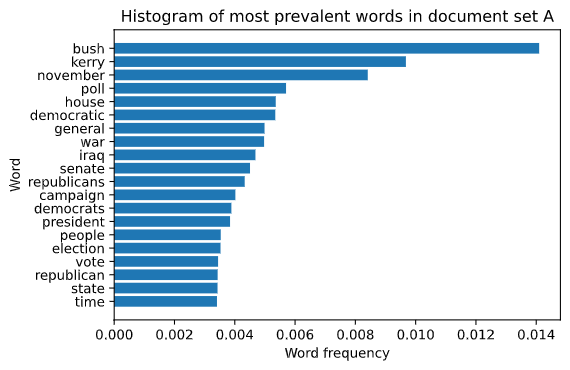
\includegraphics[width=\linewidth]{hist-ml.png}
		\caption{Top 20 most prevalent words}
		\label{fig:hist-ml-max}
	\end{subfigure}
	\begin{subfigure}{0.5\linewidth}
		\centering
		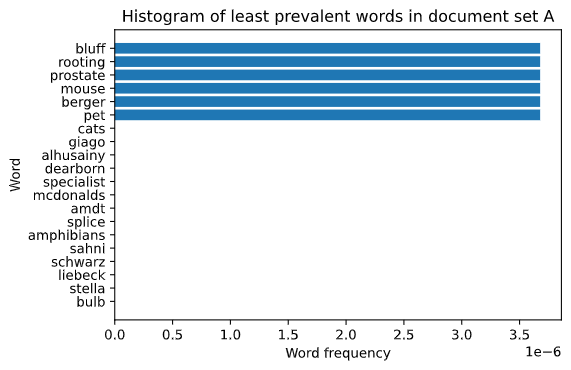
\includegraphics[width=\linewidth]{hist-ml-min.png}
		\caption{Top 20 least prevalent words}
		\label{fig:hist-ml-min}
	\end{subfigure}
	\caption{ML estimate of word probabilities trained on set $\Acal$}
	\label{fig:hist-ml}
\end{figure}
%
Figure \ref{fig:hist-ml-max} shows the empirical frequencies of the top 20 words in document set $\Acal$. We have that $\betaml_{\max} \coloneqq \frac{\max_i c_i}{C} = \frac{3833}{271898}$ for the word \textit{``bush''} (the president - not the foliage). Likewise $\betaml_{\min} \coloneqq \frac{\min c_i}{C} = 0$ as there are some words in the vocabulary $\Mcal$ that never appear in the training set $\Acal$ (such as \textit{``bulb''} in \ref{fig:hist-ml-min}). Indeed, each new word $w^*$ under ML is assumed to be drawn from:
%
\begin{equation}
	P(w^* = i | \betaml) = \frac{c_i}{C}
	\label{eqn:ml-est}
\end{equation}
%
Therefore, if we have an arbitrary test set $\mathcal{T}$ that is $T$ words long. The maximum probability test set would be $T$ repetitions of \textit{``bush''}. The lowest probability test set need only have a single word with zero probability under our ML estimate (e.g. \textit{``bulb''}) to make the probability of the whole multiply to 0.
%
\begin{align}
	\log P(\mathcal{T}) |_{\max} &= T \log \betaml_{\max} = T \log \frac{3833}{271898} \\
	\log P(\mathcal{T}) |_{\min} &= \log 0 = - \infty
\end{align}
%
This is clearly unsatisfactory; a feasible test set should not have zero probability. Therefore, the ML estimate is insufficient.
 
\subsection{Bayesian Inference}

Instead, we can perform Bayesian inference to ameliorate these issues. We assume the probability vector $\beta$ has a Dirichlet prior $\beta \sim Dir(\beta ; \alpha)$ with concentration parameter $\alpha$ - where $\alpha$ and $\beta$ are the same shape. We perform Bayesian inference to obtain the posterior for $\beta$.
%
\begin{align}
	P(\beta | \Acal) &\propto P(\beta) \cdot P(\Acal | \beta) \nonumber \\
	&= \left( \frac{1}{B(\alpha)} \prod_{m = 1}^{M} \beta_m^{\alpha_m -1} \right) \cdot \prod_{p=1}^{M} \beta_m^{c_m} \nonumber \\
	&\propto \prod_{m = 1}^{M} \beta_m^{(\alpha_m + c_m) -1} \nonumber \\
	&\propto Dir(\beta ; \alpha + c) \nonumber \\
	\therefore P(\beta | \Acal) &= Dir(\beta ; \alpha + c)
	\label{eqn:posterior}
\end{align}
%
Where, $c$ is now a vector of word counts. We say that the Dirichlet distribution is a conjugate prior to the categorical / multinomial distribution because the posterior is also Dirichlet (albeit with a new parameter). We now seek to compute the predictive distribution for a new word $w^*$ given the posterior.
%
\begin{align}
\begin{split}
	P(w^* = i | \Acal) &= \int_{\beta} P(w^* = i, \beta | \Acal) d\beta \\
	&= \int_{\beta_i} P(w^* = i | \beta , \Acal) \int_{\beta_{\backslash i}} P(\beta | \Acal) d\beta_{\backslash i} d\beta_i \\
	&= \int P(w^* = i | \beta_i) P(\beta_i | \Acal) d\beta_i \\
	&= \int \beta_i P(\beta_i | \Acal) d\beta_i \\
	&= \Expect_{\beta_i | \Acal} [\beta_i] \\
	&= \frac{\alpha_i + c_i}{\sum_{m=1}^{M} \alpha_m + c_m} \coloneqq \hat{\beta}^*_i
\end{split}
\end{align}
%
Where the last line is a simple property of the Dirichlet: the mean of each component is proportional to the corresponding parameter value (subject to normalisation). An interesting observation is that the predictive distribution is exactly equal to that computed using the MAP estimate ($\hat{\beta}^* = \hat{\beta}^{MAP}$). If we consider only a symmetric Dirichlet such that $\alpha = a \mathbf{1}$. The previous expression reduces to:
%
\begin{equation}
	P(w^* = i | \Acal) = \frac{a + c_i}{Ma + C}
	\label{eqn:pred-bayes}
\end{equation}
%
By comparing equations \ref{eqn:ml-est} and \ref{eqn:pred-bayes}, we see that the posterior has the effect of adding a pseudo-count $a$ to each word prior to observing the training set $\Acal$.
%
\begin{align}
\begin{split}
	P(w^*=i | \Acal) &> P(w^*=i | \betaml) \\
	\frac{a + c_i}{Ma + C} &> \frac{c_i}{C} \\
	Ca + Cc_i &> Mac_i + Cc_i \\
	c_i &< \frac{C}{M}
\end{split}
\end{align}
%
As the prior is symmetric the same pseudo-count $a$ is added to each word. Those with $c_i < C/M$ gain probability and those with $c_i > C/M$ lose it. The effect is that all word probabilities are drawn closer to $C/M$ but importantly no probability rank orderings stay the same. The larger the value of $a$, the stronger this effect and the less importance is assigned to the frequency observations in $\Acal$.

\subsection{Testing Performance of Bayesian Predictor}

We now apply this Bayesian analysis to an unseen test document. The log probability of all words in a document $d$ is denoted by $\{w^*_{nd}\}_{n=1}^{N_d}$. To compute the log probability $l(d)$:
%
\begin{align}
\begin{split}
	l(d) &\coloneqq \log P(\{w^*_{nd}\}_{n=1}^{N_d} | \Acal) \\
	&= \log \prod_{n=1}^{N_d} P(w^*_{nd} | \Acal) \\
	&= \log \prod_{m = 1}^{M} P(w^*=m | \Acal)^{c^*_{md}} \\
	&= \sum_{m=1}^{M} c^*_{md} \log P(w^* = m | \Acal) \\
	&= \sum_{m=1}^{M} c^*_{md} \log \frac{a+c_m}{Ma+C} \\
	&= (c^*_d)^T \log \hat{\beta}^{*}
\end{split}
\label{eqn:test-doc-prob}
\end{align}
%
Where $c^*_{md}$ is the count of word $m$ in the unseen document $d$. All words are independent, hence how we can factorise the first line. Word order matters. Therefore, we treat a document as a sequence of categorical r.v.'s rather than a single multinomial over word counts; we omit a combinatoric term for all the various permutations of words in a document. The phrase \textit{``Bush beats Kerry''} is very different to \textit{``Kerry beats Bush''} so we treat each phrase as a separate document rather than combining their probabilities.

 We set the pseudo-count parameter to $a=0.1$ (there is no integer requirement) and apply equation \ref{eqn:test-doc-prob} to test document $d=2001$, to obtain:
 %
 \begin{equation}
 	l(d=2001)|_{a=0.1} = -3691.2
 \end{equation}
 %
 As well as the log probability of document $d$, we are interested in the per-word perplexity $p(d)$ defined in equation \ref{eqn:perplex}.
%
\begin{equation}
p(d) \coloneqq \exp \left(- \frac{l(d)}{N_d} \right)
\label{eqn:perplex}
\end{equation}
%
The expected perplexity of rolls from an $n$-sided die is $n$ and so the expected perplexity for samples drawn from a uniform multinomial with $M$ total categories would be $M$. This is the maximum perplexity of a multinomial with $M$ categories as we have maximum uncertainty. We can compute the perplexities for a single document or for all documents by simply concatenating documents after one another. The results are given in table \ref{tab:perplex}.
%
\begin{table}[!h]
	\centering
	\begin{tabular}{c | c c c}
		& One doc $d=2001 \in \Bcal$ & All docs $\forall d \in \Bcal$ & Uniform multinomial \\ \hline
		per-word perplexity & 4399.0 & 2697.1 & $M=6906$
	\end{tabular}
\caption{Perplexities of documents in test set $\Bcal$ ($a=0.1$)}
\label{tab:perplex}
\end{table}
%
Documents with a higher prevalence of common words have higher log-probability and hence lower perplexity. Indeed document $d=2001$ has a higher perplexity than the average in set $\Bcal$ so we conclude that this document contain rarer words than in the rest of the set.

\subsection{Bayesian Mixture Model (BMM)}

We extend our model by introducing the concept of document categories. We define $K$ distinct categories and for each document $d$ we define a new latent variable $z_d \in \{1 \dots K\}$ denoting class membership. We assume the class memberships are drawn from a categorical distribution: $z_d \sim Cat(\theta)$ where the parameter $\theta$ has Dirichlet prior with concentration $\alpha$\footnote{Note that we are using new notation in this section. $\alpha$ is now the Dirichlet parameter over categories and $\gamma$ takes the role of Dirichlet parameter over words.} Each document category $k$ has now a different vector $\beta_k$ from which words are drawn categorically: $(w_{nd} | z_d = k) \sim Cat(\beta_k)$. Each $\beta_k$ has prior $\beta_k \sim Dir(\gamma)$. This model is summarised in figure \ref{fig:bayesian-mixture}.
%
\begin{figure}[!h]
	\centering
	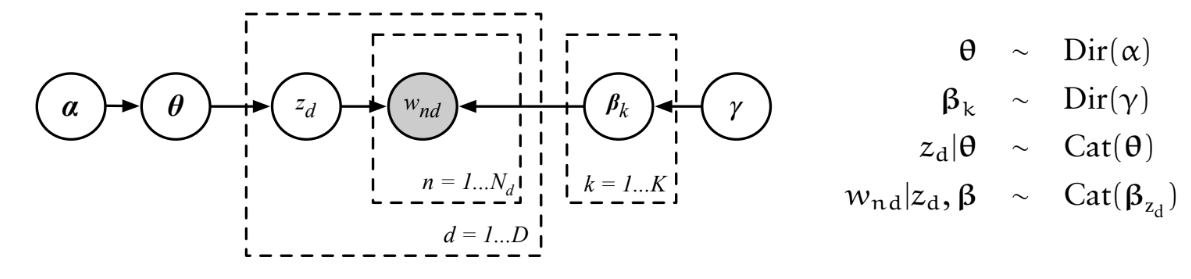
\includegraphics[width=\figwidth]{bayesian-mixture.png}
	\caption{Bayesian Mixture Model (Mixture of Multinomials)}
	\label{fig:bayesian-mixture}
\end{figure}

We choose uniform Dirichlet priors parameters $\alpha_i = 10, \gamma_i = 0.1 \enspace \forall i$ and perform Gibbs sampling using the training set $\Acal$ to obtain samples for $\theta$, $z_d$ and $\beta_k$. We plot the topic posterior as a function of Gibbs iteration $i$. This is simply the fraction of $\{z_d^{(i)}\}_{d=1}^{D}$ assigned to topic k:
%
\begin{equation}
	\theta^{(i)}_k \approx \frac{1}{D} \sum_{d=1}^{D} \mathbbm{1}(z^{(i)}_d = k)
	\label{eqn:bmm-topic-post}
\end{equation}

The results are given in figure \ref{fig:gibbs-posterior}. We see that only a handful of categories have high posterior proportions. This suggests that our value of $K=20$ is unnecessarily high. 
%
\begin{figure}[!h]
	\begin{subfigure}{0.33\linewidth}
		\centering
		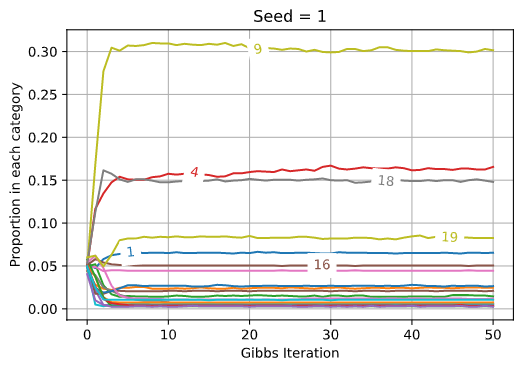
\includegraphics[width=\linewidth]{gibbs-posterior-1.png}
		\caption{Seed = 1}	
	\end{subfigure}
	\begin{subfigure}{0.33\linewidth}
		\centering
		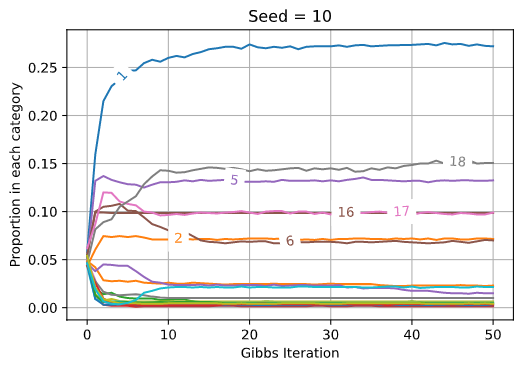
\includegraphics[width=\linewidth]{gibbs-posterior-2.png}
		\caption{Seed =	10}
	\end{subfigure}
	\begin{subfigure}{0.33\linewidth}
		\centering
		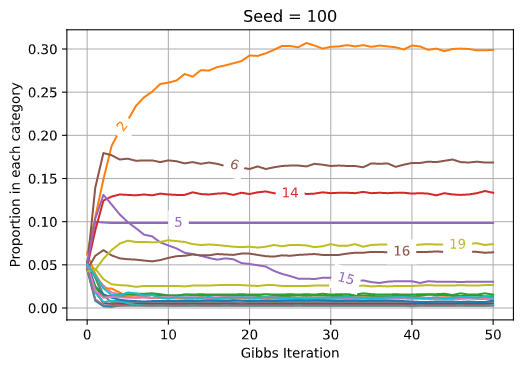
\includegraphics[width=\linewidth]{gibbs-posterior-3.png}
		\caption{Seed = 100}	
	\end{subfigure}
	\caption{BMM - Posterior over categories against Gibbs iteration for various initialisations}
	\label{fig:gibbs-posterior}
\end{figure}

Furthermore, different initialisations (seeds) yield different stationary distributions. All three Gibbs processes in figure \ref{fig:bayesian-mixture} converge well enough after 30 iterations, however the exact distribution they converge to is different - even after an arbitrary relabelling of categories. The forms of the posterior are in each case different so we cannot say that we converge to the "true" posterior but rather a local optimum that is in some sense "good enough".

\subsection{Latent Dirichlet Allocation (LDA)}

We make one final extension to our model. Now each document can be an arbitrary blend of the $K$ topics. Now every $n$th word in each document $d$ has its own topic $z_{nd} \sim Dir(\theta_d)$ and the per document topic proportions parameter $\theta_d$ is specific to each document. This extension is summarised in figure \ref{fig:lda-model}.
%
\begin{figure}[!h]
	\centering
	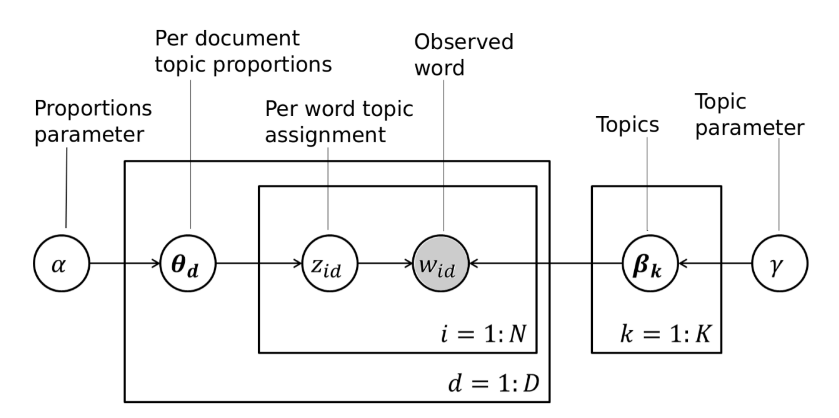
\includegraphics[width=\figwidth]{lda.png}
	\caption{Latent Dirichlet Allocation model (LDA)}
	\label{fig:lda-model}
\end{figure}

Now each document can have a mixture of topics drawn from $\theta_d$. Each document's topic posterior can be empirically calculated from the Gibbs samples (in a similar way to equation \ref{eqn:bmm-topic-post}):
%
\begin{equation}
	[\theta^{(i)}_d]_k = \frac{1}{N_d} \sum_{n=1}^{N_d} \mathbbm{1}(z^{(i)}_{nd} = k)
\end{equation}

We can now compare the computed perplexities for the test set $\Bcal$ for each of the methods outlined so far (table \ref{tab:perplex-comp}). As the models get more sophisticated (left to right), the perplexity increases as the test set $\Bcal$ has higher overall log-likelihood. A model with more degrees of freedom will always fit the training set better but it is reassuring to note that we are not over-fitting as performance still improves on unseen test data.

\begin{table}[!h]
	\centering
	\begin{tabular}{c | c c c c c}
		& Maximum Likelihood & Simple Bayes Predictive & BMM (seed=100) & LDA (seed = 1) \\ \hline
		Perplexity & $\infty$ & 2697.1 & 2100.7 & 2072.5 
	\end{tabular}
\caption{Test set $\Bcal$ perplexity (50 Gibbs iterations used for BMM and LDA)}
\label{tab:perplex-comp}
\end{table}

We can compute the word entropy for each category simply:
%
\begin{equation}
	H(w^* | z^* = k) \approx \sum_{m=1}^{M} \beta_{km} \log \frac{1}{\beta_{km}} = - \beta_k^T \log \beta_k
\end{equation}

If we choose $\log$ to be the natural logarithm then this entropy would be in units of nats. Base 2 would give us familiar bits. We choose to work in nats as that gives us easier comparison with the perplexity. Indeed, the expected value of the perplexity for a document drawn from a single topic is the exponential of the entropy as shown below:
%
\begin{align}
\begin{split}
	\log(p(d|z=k)) &= - \frac{1}{N_d} l(d) \\
	&= - \frac{1}{N_d} \sum_{m=1}^{M} c_m \log \beta_{km} \\
	\therefore \Expect [\log(p(d|z=k))] &= \sum_{m=1}^{M} \Expect \left[ \frac{c_m}{N_d} \right] \log \frac{1}{\beta_{km}} \\
	&= \sum_{m=1}^{M} \beta_{km} \log \frac{1}{\beta_{km}} \\
	&= H(w^* | z^* = k)
\end{split}
\end{align}

We plot the word entropy of each topic as a function of Gibbs iteration.

\textbf{Words}: XX

\end{document}
